\documentclass[a4paper,15pt]{article}

%Packages:
\usepackage[utf8]{inputenc}    
\usepackage[vietnamese]{babel} 
\usepackage{graphicx}          
\usepackage{amsmath , amsfonts , amssymb , amsthm} 
\usepackage{hyperref}          
\usepackage{geometry}    
\usepackage{framed}
\usepackage{float}
\usepackage{array}
\usepackage{fancyhdr}
\usepackage{lastpage} % để lấy tổng số trang
\pagestyle{fancy}
\fancyhf{}
\renewcommand{\footrulewidth}{0.4pt}

\fancyfoot[L]{Báo cáo bài tập lớn môn Vật lý bán dẫn nhóm 14 - HK242.}

% Chân trang bên phải
\fancyfoot[R]{Trang \thepage/\pageref{LastPage}}

\begin{document}
%Trang bìa
\begin{titlepage}
    \centering
    {\textbf{ĐẠI HỌC QUỐC GIA THÀNH PHỐ HỒ CHÍ MINH}} \\   
    {\textbf{TRƯỜNG ĐẠI HỌC BÁCH KHOA}} \\   
    {\textbf{KHOA ĐIỆN - ĐIỆN TỬ}} \\
    {\textbf{BỘ MÔN ĐIỆN TỬ}}\\
%Chèn logo BK    
\begin{figure}[h]
    \centering
    
\includegraphics[width=0.6\textwidth]{img/Bach khoa.png}
\end{figure}
%Title
    {\textbf{BÁO CÁO BÀI TẬP LỚN MÔN VẬT LÝ BÁN DẪN (EE1007)}} \\
    \vspace{0.5cm}
    {\huge \textbf{Tìm hiểu về mạch chỉnh lưu AC/DC.}} \\
    \hrulefill \\
    
    { \textbf{GVHD: ThS. Võ Tấn Thông}} \\
    { \textbf{Nhóm: 14}} \\
    \vspace{0.5cm}

\begin{tabular}{|m{1cm}|m{3cm}|m{3cm}|m{2cm}|}
\hline
STT & Họ và đệm  & Tên &  MSSV \\ \hline
1 & Nguyễn Thái & Hưng & 0000000 \\ \hline
\end{tabular}
\vspace{7cm} \\
\textbf{Thành phố Hồ Chí Minh, tháng 5 năm 2025}
\end{titlepage}

%Muc luc
\tableofcontents
\newpage

%Mo dau
\section{Mở đầu}
\subsection{Lời cảm ơn}
Nhóm em xin gửi lời cảm ơn chân thành nhất đến thầy Võ Tấn Thông đã hướng dẫn và hỗ trợ trong quá trình thực hiện bài báo cáo bài tập lớn này. Bài báo cáo đã giúp chúng em hiểu sâu hơn về các khái niệm và nguyên lý liên quan đến đề tài của chúng em nói riêng và môn Vật lý bán dẫn nói chung. Ngoài ra còn giúp chúng em phát triển kỹ năng nghiên cứu, thực hiện thiết kế mạch và trình bày báo cáo. \\
Chúng em rất trân trọng sự quan tâm và hỗ trợ của thầy trong quá trình học và thực hiện đề tài này. Mong rằng bài báo cáo lần này của chúng em đã đáp ứng được những kỳ vọng và yêu cầu của thầy. Chúng em biết rằng bài báo cáo này vẫn sẽ còn nhiều khuyết điểm và thiếu sót. Vì thế chúng em sẵn sàng nhận được sự góp ý và lắng nghe phản hồi của thầy để giúp chúng em hoàn thiện hơn.\\
Lời cuối cùng, chúng em xin cảm ơn thầy và chúc thầy nhiều sức khoẻ và đạt được nhiều thành công.


\subsection{Giới thiệu về đề tài}
Trong đời sống hiện đại và trong các hệ thống điện – điện tử, nhu cầu chuyển đổi dòng điện xoay chiều (AC) sang dòng điện một chiều (DC) là vô cùng cần thiết. Hầu hết các thiết bị điện tử như máy tính, điện thoại, tivi, bộ sạc, thiết bị công nghiệp,... đều hoạt động nhờ dòng điện một chiều được cung cấp thông qua các mạch nguồn. Thành phần quan trọng và không thể thiếu trong các mạch nguồn này chính là mạch chỉnh lưu AC/DC. Ở đề tài này, chúng em sẽ thực hiện các vấn đề sau:
\begin{itemize}
    \item Nắm vững kiến thức cơ bản về dòng điện AC, DC.
    \item Tìm hiểu về các mạch chỉnh lưu: bán kỳ, toàn kỳ dùng 2 diode, mạch chỉnh lưu cầu,...
    \item Thiết kế, mô phỏng lại một loại mạch chỉnh lưu.
\end{itemize}
\newpage

\section{Cơ sở lý thuyết}
\subsection{Giới thiệu}
\subsubsection{Khái niệm}
Mạch chỉnh lưu là mạch điện dùng để chuyển đổi dòng điện xoay chiều thành dòng điện một chiều. Quá trình này được thực hiện chủ yếu thông qua các linh kiện bán dẫn như diode, thyristor, SCR, kết hợp với các linh kiện lọc như tụ điện và cuộn cảm để làm giảm gợn sóng và ổn định điện áp đầu ra.\\
Nguyên lý hoạt động của mạch chỉnh lưu dựa trên đặc tính của diode, một linh kiện điện tử chỉ cho phép dòng điện đi qua nó theo một chiều nhất định. Khi một diode được mắc nối tiếp với nguồn điện xoay chiều, ở nửa chu kỳ dương, diode sẽ được phân cực thuận và dòng điện sẽ đi qua diode theo chiều dương. Ở nửa chu kỳ âm, diode sẽ bị phân cực ngược và dòng điện sẽ không đi qua diode. Do đó, ở đầu ra của mạch chỉnh lưu, chỉ có nửa chu kỳ dương của dòng điện xoay chiều được giữ lại, tạo thành dòng điện một chiều.\\
Chúng ta có thể dễ dàng tìm thấy mạch chỉnh lưu trong các thiết bị điện tử ở chính gia đình của mình như tivi, máy lạnh, bộ sạc điện thoại,... hoặc trong các thiết bị công nghiệp như máy hàn, khởi động mềm,... Và mạch chỉnh lưu có một số chức năng như sau:
\begin{itemize}
    \item Làm nguồn điện một chiều để điều khiển cho các thiết bị mạ, hàn một chiều.
    \item Là nguồn điện cho một số động cơ điện một chiều, mạch chỉnh lưu sẽ cung cấp cho mạch kích từ của máy điện một chiều hoặc máy điện đồng bộ.
    \item Ứng dụng trong trong các bộ chuyển đổi điện xoay chiều thành điện một chiều để truyền tải đi xa.
    \item Trong các thiết bị biến tần Inverter mạch chỉnh lưu được dùng để truyền động điện động cơ xoay chiều.
\end{itemize}
\subsubsection{Giới thiệu một số loại mạch chỉnh lưu}
Tuỳ thuộc vào yêu cầu của tải hiện tại mà có thể lụa chọn mạch chỉnh lưu phù hợp. Có các loại mạch chỉnh lưu phổ biến như sau:
\begin{itemize}
    \item Mạch chỉnh lưu bán kỳ (nửa chu kỳ): Sử dụng một diode để chỉ cho phép một nửa chu kỳ của dòng điện xoay chiều (AC) chuyển thành dòng điện một chiều (DC). 
    \item Mạch chỉnh lưu toàn kỳ dùng 2 diode: Gồm 2 diode để chỉnh lưu cả hai nửa chu kỳ của dòng điện xoay chiều (AC) chuyển thành dòng điện một chiêu (DC) từ toàn bộ tín hiệu AC.
    \item Mạch chỉnh lưu cầu: Sử dụng 4 diode trong một cấu hình cầu để chỉnh lưu cả hai nửa chu kỳ của dòng AC.
\end{itemize}
\newpage
\subsection{Các loại mạch chỉnh lưu}
\subsubsection{Mạch chỉnh lưu bán kỳ}
\begin{figure}[H]
    \centering
    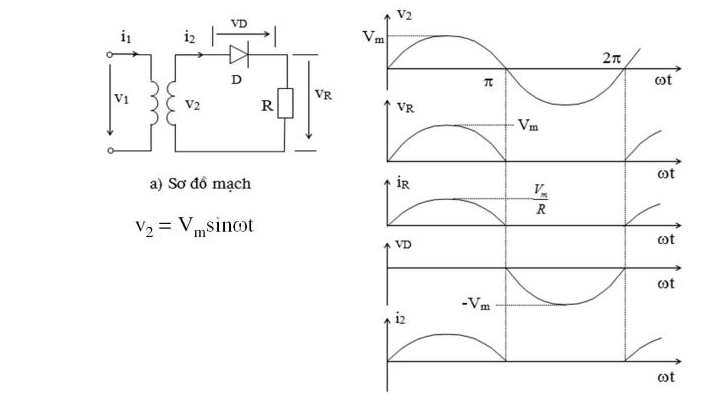
\includegraphics[scale=0.7]{img/sodomachbanky.PNG}
    \caption{Các thông tin về mạch chỉnh lưu bán kỳ}
    \label{fig:enter-label}
\end{figure}

Nguyên lý hoạt động của mạch chỉnh lưu bán kỳ:
\begin{itemize}
    \item Giai đoạn 1 – Nửa chu kỳ dương: Khi sóng AC có điện áp dương (0° đến 180°), diode dẫn dòng điện. Dòng điện đi qua tải, tạo ra điện áp DC dạng xung tại đầu ra.
    \item Giai đoạn 2 – Nửa chu kỳ âm: Khi sóng AC chuyển sang điện áp âm (180° đến 360°), diode chặn dòng điện. Kết quả là không có dòng điện đi qua tải trong giai đoạn này.
    \item Dòng điện đầu ra có dạng xung, chỉ tồn tại trong nửa chu kỳ dương của sóng AC. Đây là tín hiệu DC không liên tục với độ ổn định thấp.
\end{itemize}
Ưu và nhược điểm của mạch chỉnh lưu bán kỳ:
\begin{itemize}
    \item Ưu điểm: thiết kế đơn giản, chi phí chế tạo thấp, kích thước nhỏ, dễ dàng sử dụng,...
    \item Nhược điểm: hiệu suất thấp, độ gợn sóng cao, điện áp trung bình thấp, không thích hợp với các thiết bị yêu cầu nguồn DC ổn định,...
\end{itemize}
Một số ứng dụng của mạch chỉnh lưu bán kỳ:
\begin{itemize}
    \item Bộ nguồn đơn giản, chi phí thấp
    \item  Mạch đèn LED chiếu sáng
    \item Mạch hàn điện mini
\end{itemize}
\newpage
\subsubsection{Mạch chỉnh lưu toàn kỳ dùng 2 diode}
\begin{figure}[H]
    \centering
    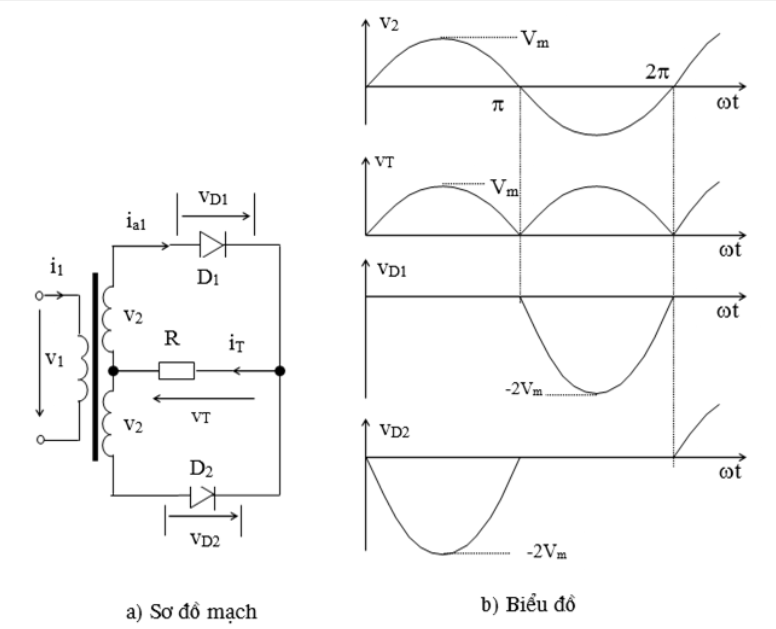
\includegraphics[scale=0.5]{img/sodomachtoanky.PNG}
    \caption{Các thông tin về mạch chỉnh lưu toàn kỳ}
    \label{fig:enter-label}
\end{figure}
Nguyên lý hoạt động của mạch chỉnh lưu toàn kỳ: 
\begin{itemize}
    \item Biến áp cung cấp điện áp xoay chiều với trung điểm chia đôi cuộn thứ cấp. Trong một chu kỳ AC, các diode D1 và D2 dẫn điện luân phiên theo chiều phân cực thuận để đưa dòng điện một chiều (DC) qua tải.
    
\end{itemize}
Ưu và nhược điểm của mạch chỉnh lưu toàn kỳ:
\begin{itemize}
    \item Máy biến áp ở đây có cấu tạo phức tạp, mỗi nửa cuộn dây thứ cấp chỉ dẫn dòng trong một bán kỳ nên công suất tính toán lớn và hiệu suất sử dụng biến áp không cao.
    \item Nhưng nhược điểm của sơ đồ là hạn chế ứng dụng trong lĩnh vực điện áp cao hoặc công suất lớn.
    \item Tuy nhiên đây là sơ đồ chỉnh lưu hai bán kỳ có số lượng điốt nhỏ nhất nên tỏ ra hiệu quả trong lĩnh vực điện áp thấp, khi đó sụt áp trên các điốt là nhỏ nhất.
\end{itemize}
Một số ứng dụng của mạch chỉnh lưu toàn kỳ:
\begin{itemize}
    \item Radio, máy phát thanh
    \item Thiết bị đo lường (VOM analog)
    \item Ứng dụng trong mạch điều khiển động cơ nhỏ, mạch relay hoặc mạch điều khiển tốc độ quạt
    \item Dùng cho các bộ sạc yêu cầu dòng nạp ổn định hơn mạch bán kỳ.
\end{itemize}
\newpage 
\subsubsection{Mạch chỉnh lưu cầu}
\begin{figure}[H]
    \centering
    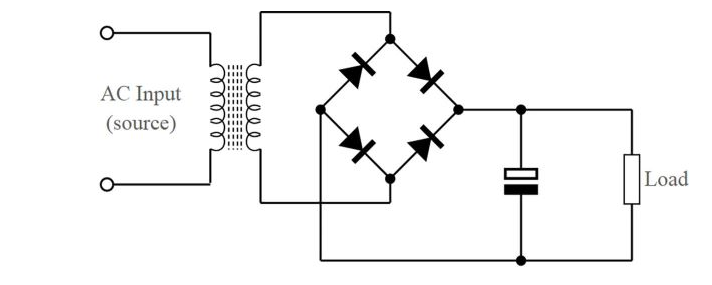
\includegraphics[scale=0.7]{img/sodomachcau.PNG}
    \caption{Sơ đồ mạch chỉnh lưu cầu}
    \label{fig:enter-label}
\end{figure}
Nguyên lý hoạt động của mạch chỉnh lưu cầu:
\begin{itemize}
    \item Trong nửa chu kỳ dương (+) của dạng sóng AC, các diode D1 và D2 được phân cực thuận, trong khi D3 và D4 bị phân cực ngược. Khi điện áp đạt đến ngưỡng dẫn của D1 và D2, dòng tải bắt đầu di chuyển.
    \item Ngược lại, trong nửa chu kỳ âm (-) của dạng sóng AC, D3 và D4 được phân cực thuận, còn D1 và D2 chuyển sang phân cực ngược. Dòng tải lúc này sẽ đi qua D3 và D4.
    \item Từ nguyên lý hoạt động trong cả hai nửa chu kỳ, ta thấy rằng dòng tải luôn có cùng hướng khi đi qua các diode. Điều này đồng nghĩa với việc dòng điện tại đầu ra luôn là dòng một chiều (DC). Nhờ bộ chỉnh lưu cầu, dòng điện xoay chiều (AC) đầu vào được chuyển đổi thành dòng điện một chiều (DC), phục vụ cho các ứng dụng yêu cầu nguồn DC ổn định.
\end{itemize}
Ưu điểm và nhược điểm của mạch chỉnh lưu cầu:
\begin{itemize}
    \item Ưu điểm: Diode không phải chịu điện áp ngược cao, dạng sống ngõ có độ gợn thấp $\rightarrow$ Dễ lọc, hiệu suất cao,...
    \item Nhược điểm: Mạch phức tạp, phải dùng đến 4 diode.
\end{itemize}
Một số ứng dụng của mạch chỉnh lưu cầu:
\begin{itemize}
    \item Bộ sạc điện thoại, laptop
    \item Nguồn máy tính để bàn (PSU)
    \item TV, amply, đầu đĩa, thiết bị gia dụng
    \item Sử dụng để nạp pin, ắc quy 6V/12V/24V vì dòng ra đều và mạnh hơn chỉnh lưu bán kỳ hoặc toàn kỳ 2 diode.
    \item Đèn LED dân dụng 220V
\end{itemize}
\newpage
\section{Thiết kế mạch chỉnh lưu}
\subsection{Chuẩn bị}
\subsubsection{Biến áp 220V $\rightarrow$ 12V}
\textbf{a. Cấu tạo, nguyên lý hoạt động}\\
Biến áp gồm hai cuộn dây sơ cấp và thứ cấp quấn trên lõi sắt từ. Khi điện áp xoay chiều 
220V được cấp vào cuộn sơ cấp, từ trường biến thiên sẽ cảm ứng điện áp ở cuộn thứ cấp 
theo tỷ lệ số vòng dây. Biến áp 12V sẽ cho ra điện áp xoay chiều hiệu dụng 12V tại đầu ra, 
dùng để cấp cho mạch chỉnh lưu.\\
\textbf{b. Ứng dụng} \\
\begin{itemize}
    \item Dùng để hạ áp điện lưới 220V xuống mức phù hợp cho thiết bị điện tử. 
    \item Bảo vệ mạch khỏi điện áp cao. 
    \item Cách ly an toàn giữa lưới điện và mạch xử lý.
\end{itemize}
\subsubsection{Diode 1N4007}
\textbf{a. Cấu tạo, nguyên lý hoạt động} \\
Diode 1N4007 là linh kiện bán dẫn có cấu trúc p-n, chỉ cho dòng điện đi qua theo một chiều 
từ cực dương (anode) sang cực âm (cathode). Trong mạch chỉnh lưu cầu, bốn diode được mắc 
thành cầu để cho phép dòng điện đi qua tải theo một chiều trong cả hai nửa chu kỳ của dòng 
xoay chiều.\\
Khi điện áp vào là AC, mỗi nửa chu kỳ sẽ có 2 trong 4 diode dẫn điện, làm cho dòng điện 
qua tải luôn cùng chiều. \\
\textbf{b. Ứng dụng}\\
Diode 1N4007 dùng để chỉnh lưu dòng điện trong các bộ nguồn AC–DC, mạch bảo vệ, mạch 
sạc, thiết bị điện tử tiêu dùng. Do chịu được điện áp ngược cao (1000V) và dòng 1A, 1N4007 
phù hợp cho nhiều ứng dụng dân dụng và công nghiệp. \\
\subsubsection{Tụ điện phân cực 470 $\mu\text{F}$}
\textbf{a. Cấu tạo, ứng dụng, nguyên lý hoạt động} \\
Tụ điện 470 $\mu\text{F}$ là tụ hóa (electrolytic capacitor), gồm hai bản cực và chất điện môi hóa học. Khi được nạp điện, tụ có khả năng lưu trữ năng lượng điện dưới dạng trường điện. Trong 
mạch chỉnh lưu, tụ được dùng để lọc điện – làm giảm độ gợn sóng sau khi điện xoay chiều 
được chỉnh lưu thành một chiều. Tụ tích điện khi điện áp tăng, và phóng điện khi điện áp 
giảm, giúp giữ điện áp đầu ra ổn định hơn. \\
Tụ 470 $\mu\text{F}$ thường dùng để làm phẳng điện áp DC trong các mạch nguồn, mạch điều khiển, 
mạch vi xử lý. Nếu tải tiêu thụ dòng nhỏ, tụ điện này là đủ để giữ cho điện áp ổn định. Với tải lớn hơn, có thể cần tăng điện dung lên 1000 $\mu\text{F}$ hoặc nhiều hơn. \\
\textbf{b. Sơ đồ} \\
\begin{figure}[H]
    \centering
    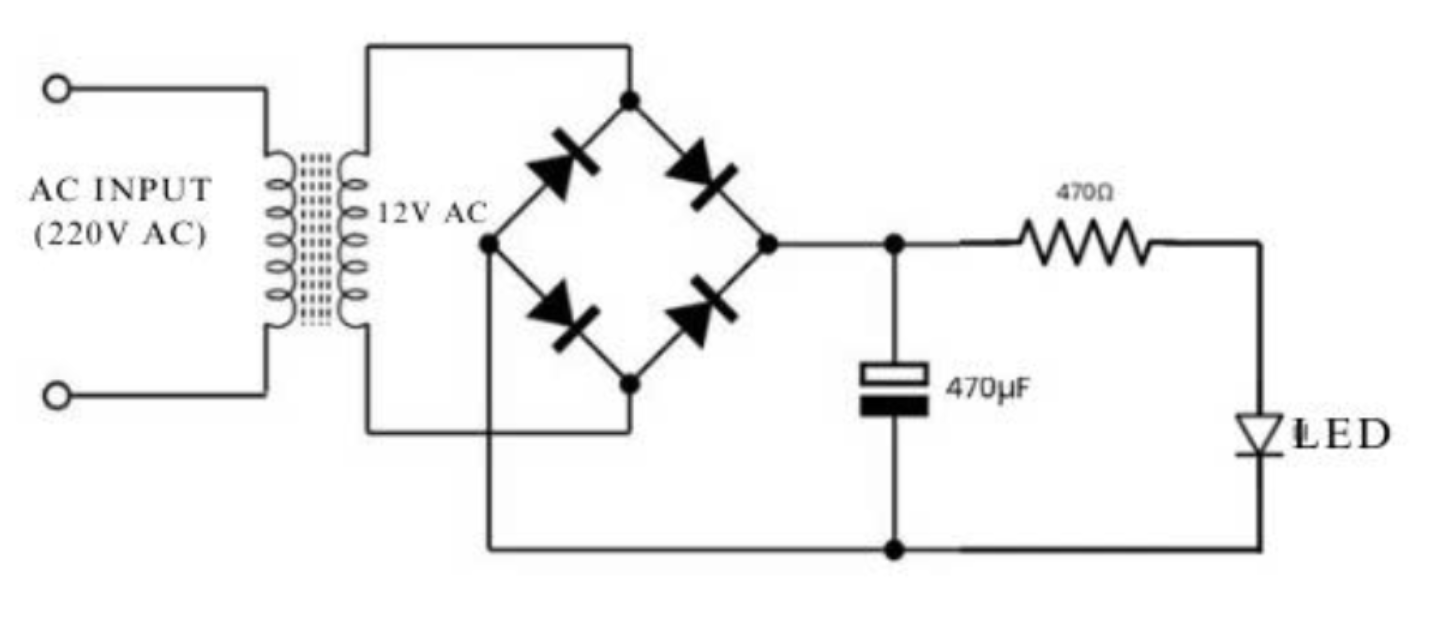
\includegraphics[scale=0.4]{img/Sodomach.png}
    \caption{Tụ điện được mắc song song với đầu ra của cầu diode}
    \label{fig:enter-label}
\end{figure}
\subsubsection{Điện trở 470$\Omega$ }
\textbf{a. Cấu tạo, Nguyên lý hoạt động} \\
Điện trở là linh kiện làm từ vật liệu có điện trở suất cao, giới hạn dòng điện trong 
mạch. Trong mạch chỉnh lưu, điện trở 470$\Omega$ thường được mắc nối tiếp với đèn LED 
để giới hạn dòng điện, tránh hỏng LED do quá dòng. \\
\[
R = \frac{V_{power}- V_{LED}}{I_{LED}} = \frac{12V - 2V}{0.02A} = 500 \Omega
\] 
Với $V_{power} = 12V $ và $V_{LED} \approx 2V$ $\rightarrow I \approx 21mA$ \\
\textbf{b. Sơ đồ} \\
\begin{figure}[H]
    \centering
    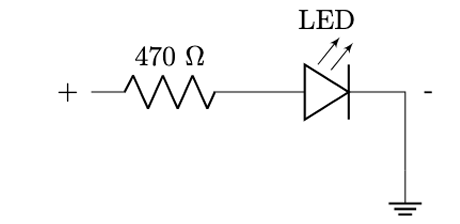
\includegraphics[scale=0.6]{img/Dientro.PNG}
    \caption{Sơ đồ điện trở nối tiếp LED}
    \label{fig:enter-label}
\end{figure}
\subsubsection{Đèn LED}
\textbf{a. Cấu tạo, nguyên lý hoạt động} \\
Là một loại diode bán dẫn phát quang. Khi dòng điện đi theo chiều thuận qua LED, các điện 
tử tái hợp với lỗ trống tạo ra ánh sáng. LED có hai chân: anode (dài hơn) và cathode (ngắn 
hơn).  \\
Trong mạch chỉnh lưu, LED được dùng làm đèn báo nguồn. Khi có điện áp DC ổn định, LED 
sáng báo hiệu mạch hoạt động.\\
\textbf{b. Ứng dụng} \\
LED được sử dụng rộng rãi làm đèn báo nguồn, đèn chiếu sáng, hiển thị trạng thái, chỉ thị 
lỗi, trang trí trong các mạch điện tử dân dụng và công nghiệp.\\
\section{Sơ đồ và mạch thực tế của mạch chỉnh lưu cầu 4 diode}
\begin{figure}[H]
    \centering
    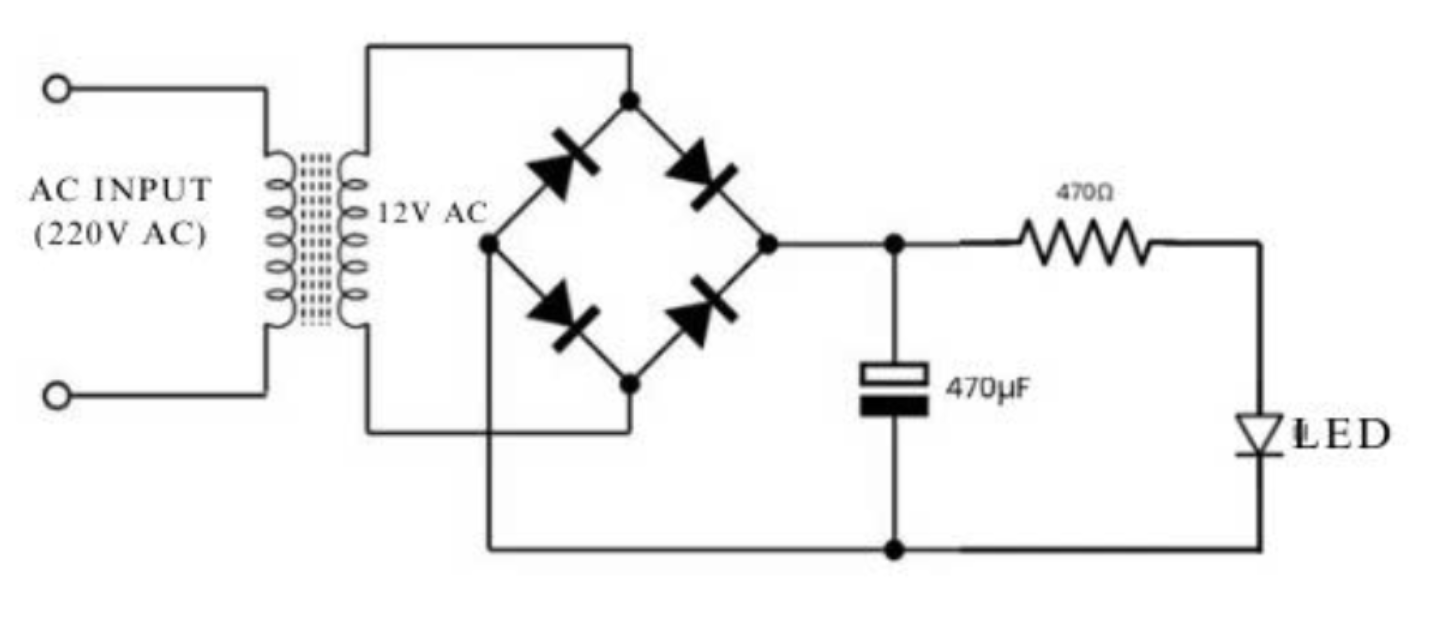
\includegraphics[scale=0.6]{img/Sodomach.png}
    \caption{Sơ đồ mạch}
    \label{fig:enter-label}
\end{figure}
\begin{figure}[H]
    \centering
    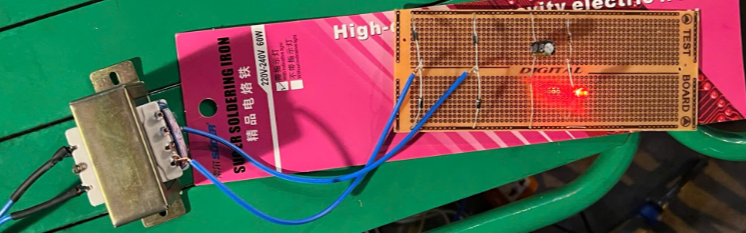
\includegraphics[scale=0.45]{img/Machthucte.PNG}
    \caption{Mạch thực tế}
    \label{fig:enter-label}
\end{figure}
\section{Ứng dụng thực tế}
Mạch chỉnh lưu cầu 4 diode là nền tảng cho hầu hết các bộ nguồn điện tử hiện nay. Trong 
thực tế, mạch được sử dụng để tạo ra nguồn điện DC cho các thiết bị điều khiển vi xử lý như 
Arduino, PIC, STM32, dùng trong các mạch cảm biến, bộ nguồn adapter, mạch sạc điện 
thoại, sạc pin dự phòng, và các bộ cấp nguồn ổn áp như LM7805, LM7812.  
Ngoài ra, mạch còn được ứng dụng trong các thiết bị dân dụng như radio, đồng hồ kỹ thuật 
số, đèn LED trang trí, máy tính mini, mạch nguồn máy in, máy fax, và nhiều hệ thống tự động 
hóa gia đình. 
Nhờ vào cấu trúc đơn giản, chi phí thấp và độ ổn định cao, mạch chỉnh lưu cầu 4 diode là 
một phần không thể thiếu trong các hệ thống điện tử dân dụng và công nghiệp. Việc hiểu rõ 
nguyên lý hoạt động cũng như cách lựa chọn các linh kiện phù hợp sẽ giúp sinh viên và kỹ 
thuật viên có nền tảng vững chắc khi thiết kế các mạch nguồn cho ứng dụng thực tế.
\section{Lời kết}
Thông qua quá trình tìm hiểu và nghiên cứu đề tài, nhóm chúng em đã tích lũy thêm nhiều kiến thức mới, đồng thời hiểu rõ hơn cách thu thập thông tin và vận dụng lý thuyết vào thực tiễn. Mặc dù vẫn còn hạn chế về kinh nghiệm và kiến thức chuyên môn, dẫn đến một số thiếu sót không thể tránh khỏi trong quá trình thực hiện, chúng em rất mong nhận được sự góp ý chân thành từ thầy/cô để có thể hoàn thiện hơn trong những lần sau.\\
Dù gặp không ít khó khăn, thử thách trong quá trình thực hiện đề tài, chúng em đã học hỏi được nhiều bài học quý báu, từ việc rèn luyện kỹ năng tìm tòi, làm việc nhóm, đến cách tổ chức công việc hiệu quả. Qua đó, mỗi thành viên đều nâng cao tinh thần trách nhiệm, nâng cao kiến thức và giúp cho chúng em càng thêm đam mê đối với ngành kỹ thuật.\\
Lời cuối, nhóm chúng em xin chân thành cảm ơn sự hướng dẫn tận tình của thầy và kính chúc thầy dồi dào sức khỏe, thành công hơn.
\newpage
\section{Tài liệu tham khảo}
\begin{thebibliography}{9}
\bibitem{hansinco}
Hansinco,
\textit{Mạch chỉnh lưu là gì? Phân loại, chức năng và công dụng},
\url{https://hansinco.com.vn/tin-tuc/mach-chinh-luu.html}
\bibitem{hansinco}
Hansinco,
\textit{Tìm hiểu về mạch chỉnh lưu cầu: cấu tạo và hoạt động},
\url{https://hansinco.com.vn/tin-tuc/mach-chinh-luu-cau.html}
\bibitem{drex}
Drex,
\textit{Rectifier Circuits 101: A Beginner’s Guide},
\url{https://www.icdrex.com/rectifier-circuits-101-a-beginners-guide/}
\bibitem{allaboutcircuits}
All About Circuits,
\textit{Rectifier Circuits},
\url{https://www.allaboutcircuits.com/textbook/semiconductors/chpt-3/rectifier-circuits/}
\bibitem{wiki}
Wikipedia,
\textit{Mạch chỉnh lưu},
\url{https://vi.wikipedia.org/wiki/M%E1%BA%A1ch_ch%E1%BB%89nh_l%C6%B0u}
\end{thebibliography}
\end{document}
